\documentclass{beamer}


\usepackage[no-math]{fontspec}
\usepackage{xunicode}
\usepackage{xltxtra}
\usepackage{tikz}
\usepackage{graphicx}
\usepackage{relalg}
\usepackage{booktabs}
\usepackage{fontawesome}
\usepackage[normalem]{ulem}
\usepackage{hyperref}


% Beamer setup
\mode<presentation>
{
	\usetheme{OtagoPlain}
	\setbeamertemplate{navigation symbols}{}
}
\setbeamertemplate{footline}[frame number]


% TikZ setup
\usetikzlibrary{positioning}
% \usetikzlibrary{graphs}
% \usetikzlibrary{decorations.pathreplacing}
\usetikzlibrary{calc}
\usetikzlibrary{arrows.meta}


% fontspec setup
\defaultfontfeatures{Mapping=tex-text}
\setmainfont{Minion Pro}
\setsansfont[Scale=MatchUppercase,BoldFont={Open Sans}]{Open Sans Light}
\setmonofont[Scale=MatchLowercase]{Letter Gothic 12 Pitch}


% graphicx setup
\graphicspath{{images/}}


% misc
\newcommand{\todo}[1]{\textbf{!!TODO!!} {[#1]}}


% Draw a grid to aid TikZ picture drawing/debugging.
\newcommand{\DrawGridTikZ}[2]{%
	\begin{scope}[color=lightgray]
		\draw[thin,step=1mm]  (0.0,0.0)   grid (#1,#2);%
		\draw[thick,step=1cm] (-0.1,-0.1) grid (#1+0.1,#2+0.1);%
		\pgftext[top,at={\pgfxy(0.0,-0.2)}]{\tiny 0}%
		\pgftext[right,at={\pgfxy(-0.2,0.0)}]{\tiny 0}%
		\foreach \x in {1,...,#1} {\pgftext[top,at={\pgfxy(\x,-0.2)}]{\tiny\x}}%
		\foreach \y in {1,...,#2} {\pgftext[right,at={\pgfxy(-0.2,\y)}]{\tiny\y}}%
	\end{scope}
}


% Sometimes we want to put a comment in tiny text on the next line, but the default line skip
% will insert too much vertical space. Put a \tinyskip at the end of the line instead.
\def\tinyskip{\\[-0.33\baselineskip]}


% Bold-face text using the structure colour.
\newcommand<>{\structurebf}[1]{\structure#2{\textbf{#1}}}


% preamble
\title{Adventures in data wrangling}
\author{Nigel Stanger}
\date{July 20, 2018}


\begin{document}


%%%%%%%%%%%%%%%%%%%%%%%%%%%%%%%%%%%%%%%%%%%%%%%%%%%%%%%%%%%%%%%%%%%%%%%%%%%%%%%%


\setbeamertemplate{background canvas}{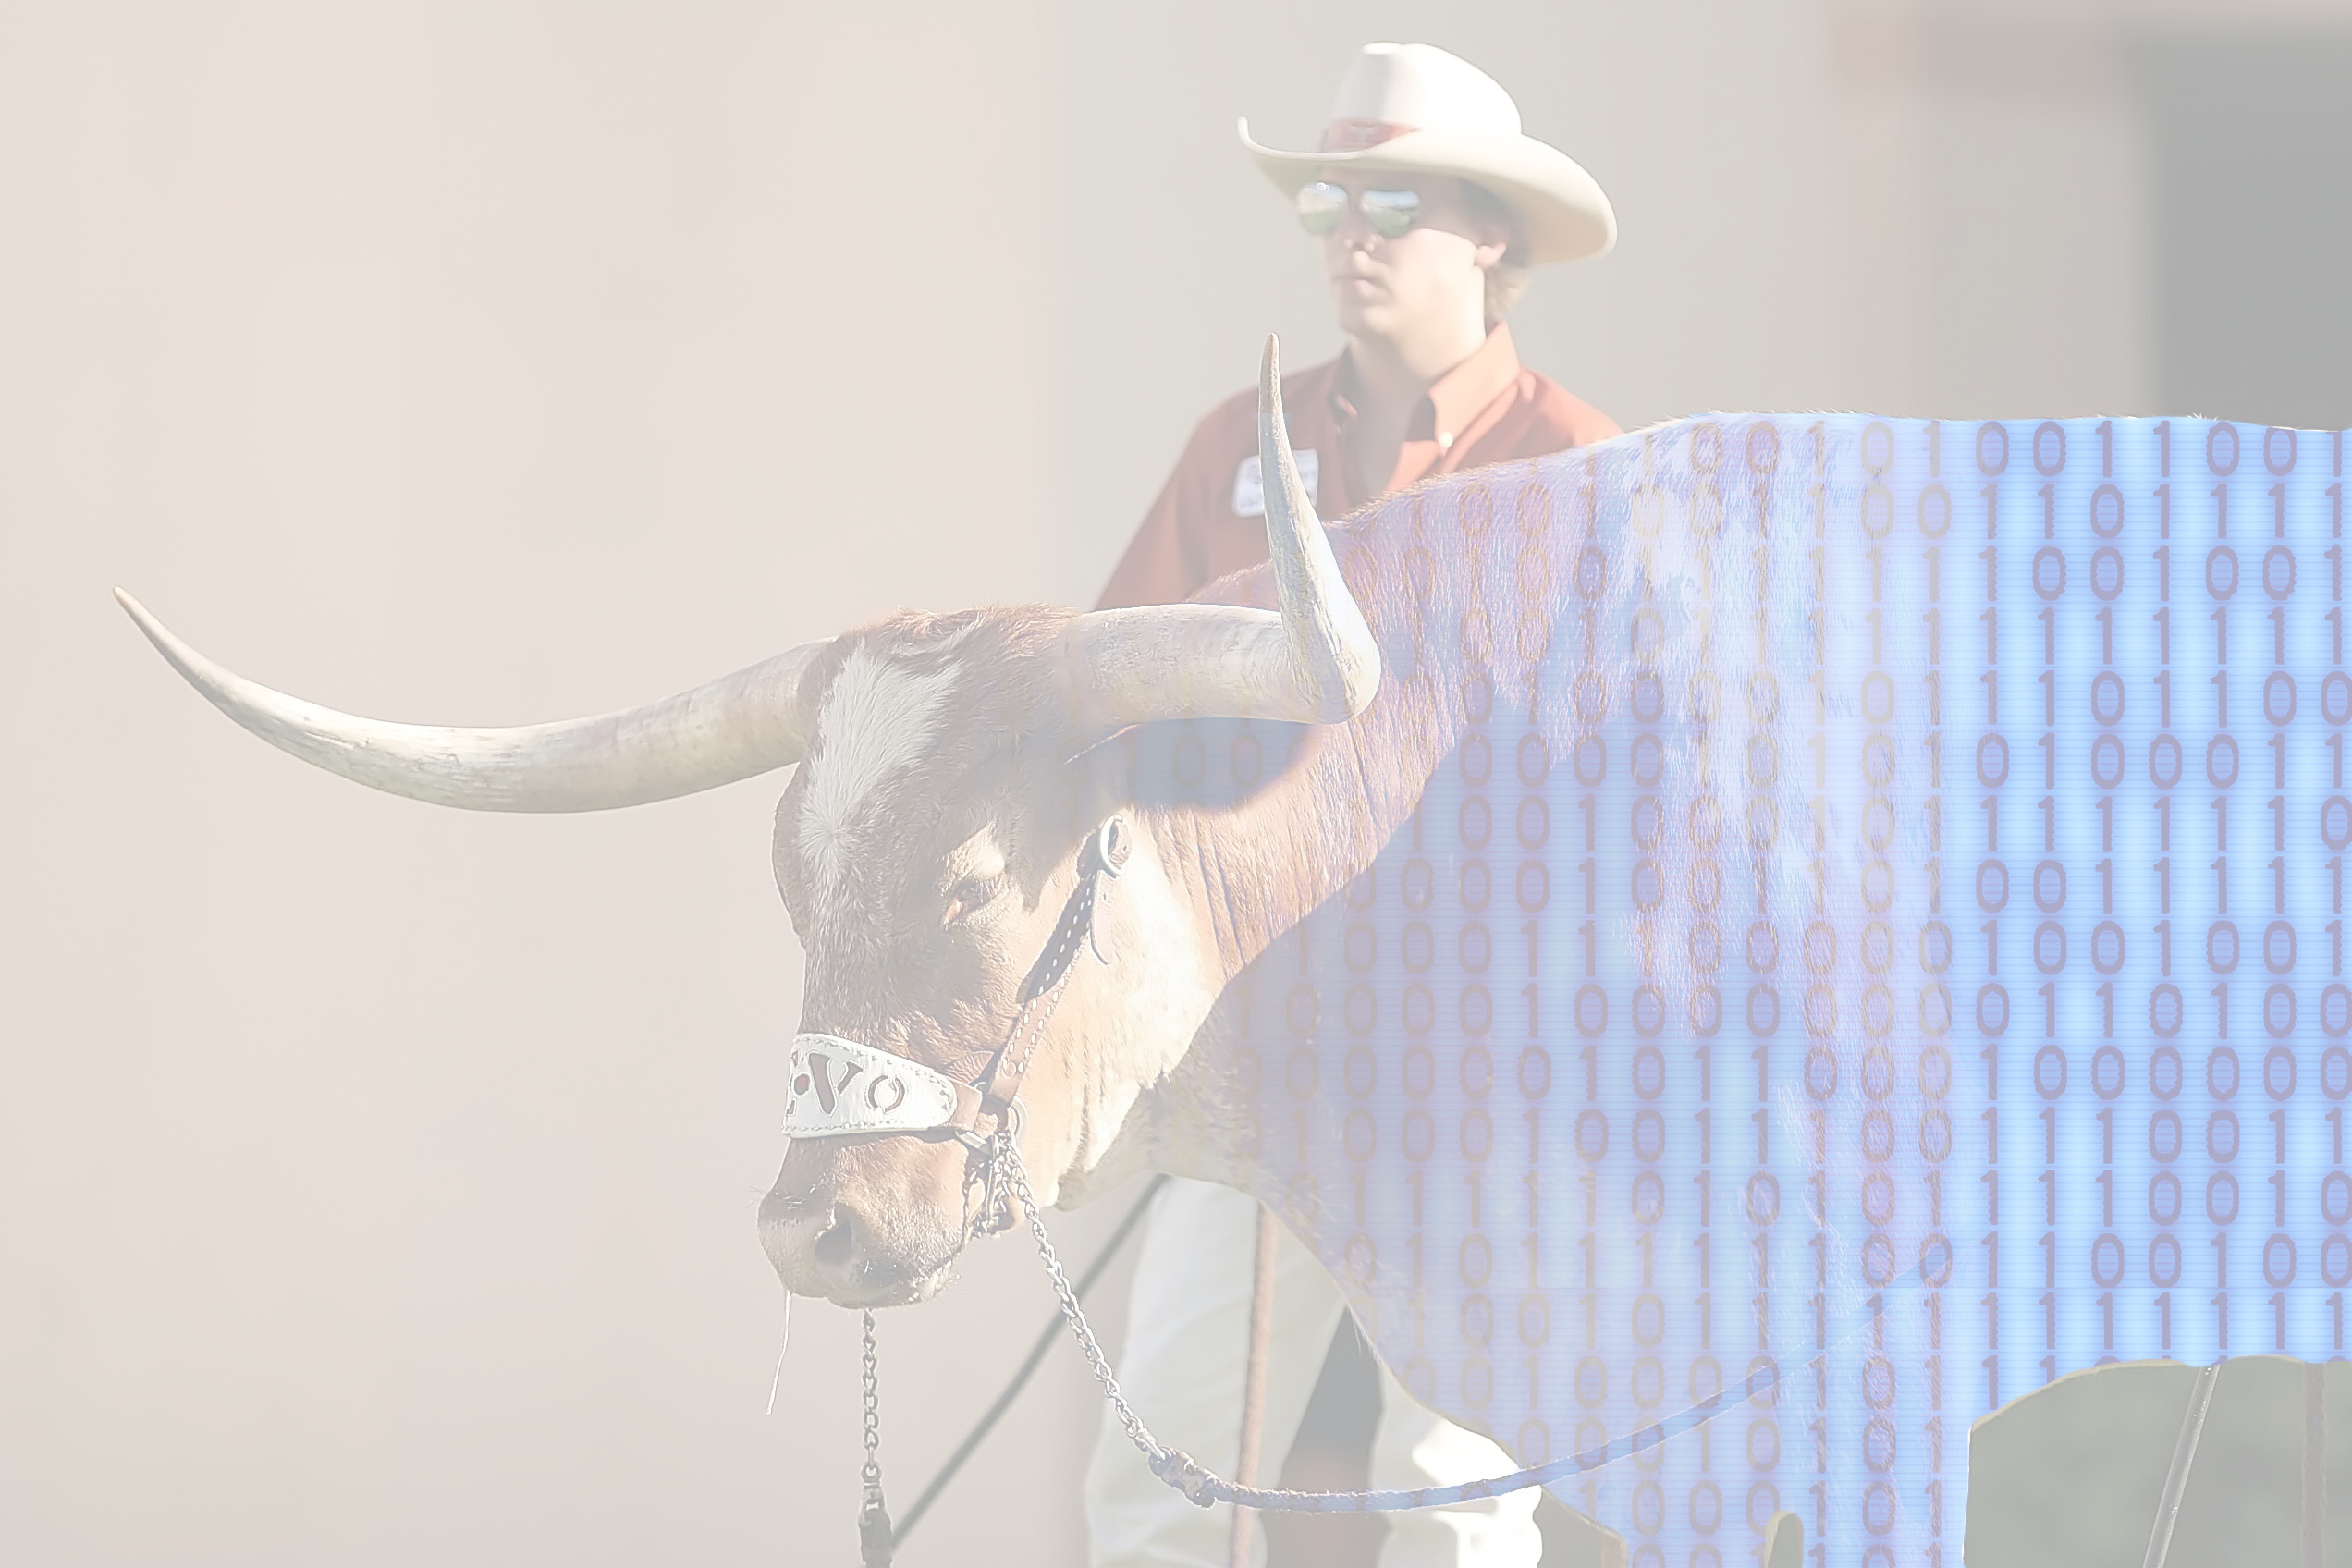
\includegraphics[height=\paperheight,keepaspectratio]{data-wrangler-BG.jpg}}
% to create image:
%   1. export data-wrangler.xcf as PNG from GIMP
%   2. convert data-wrangler.png -fill white -colorize 67% data-wrangler-bg.jpg

\begin{frame}
    \thispagestyle{empty}
    \titlepage
\end{frame}

\setbeamertemplate{background canvas}[default]


%%%%%%%%%%%%%%%%%%%%%%%%%%%%%%%%%%%%%%%%%%%%%%%%%%%%%%%%%%%%%%%%%%%%%%%%%%%%%%%%


\setbeamertemplate{background canvas}{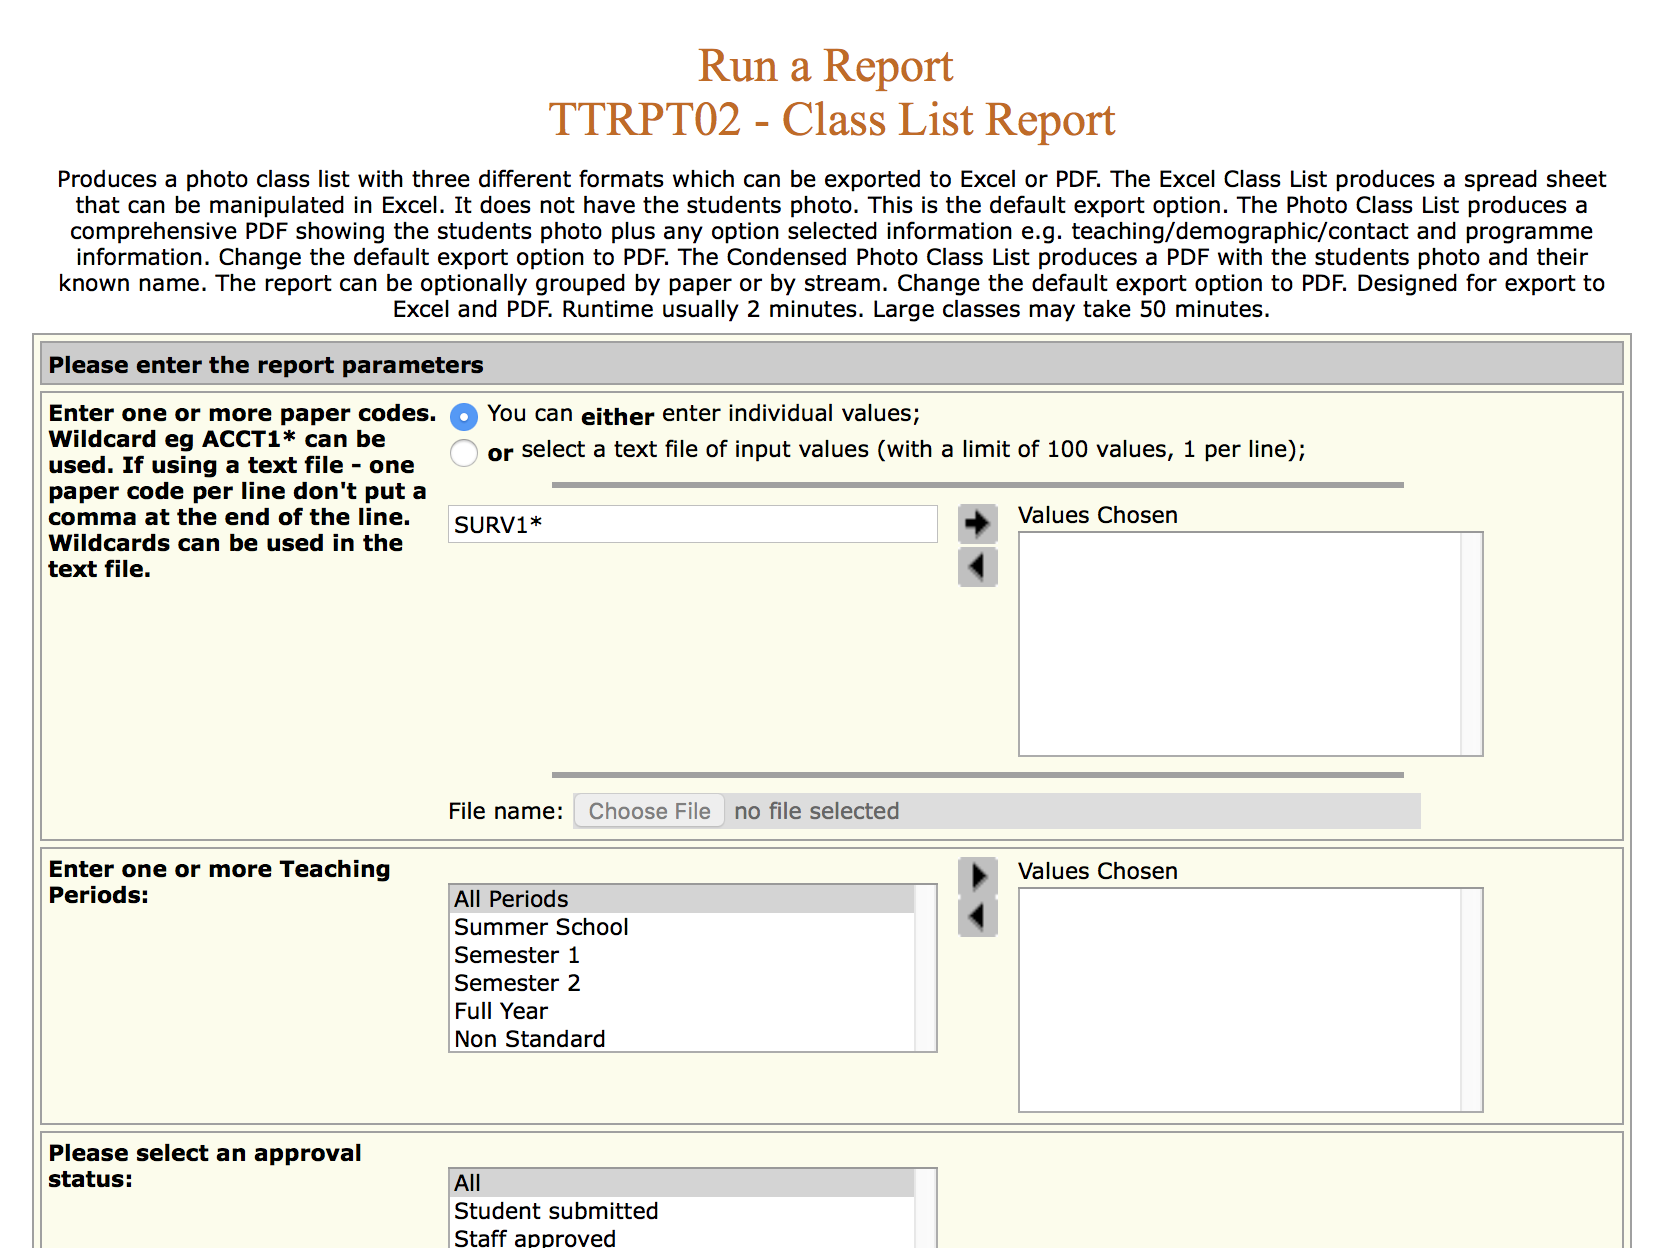
\includegraphics[width=\paperwidth,keepaspectratio]{TTRPT02.png}}

\begin{frame}
    \thispagestyle{empty}
\end{frame}

\setbeamertemplate{background canvas}[default]


%%%%%%%%%%%%%%%%%%%%%%%%%%%%%%%%%%%%%%%%%%%%%%%%%%%%%%%%%%%%%%%%%%%%%%%%%%%%%%%%


\begin{frame}
    \frametitle{Data come from a \uline{lot} of different sources}
    
    \bigskip
    \begin{columns}
        \begin{column}{0.4\paperwidth}
            \centering
            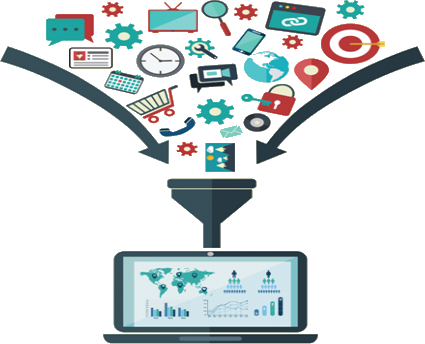
\includegraphics[width=0.9\columnwidth,keepaspectratio]{data-sources.png}\tinyskip
            {\tiny{SOURCE: Xobber}}
        \end{column}
        \begin{column}{0.55\paperwidth}
            \centering
            \begin{tabular}{cccccccc}
                \faHeartO & \faCode & \faDatabase & \faGit & \faCalendar & \faLaptop & \faThumbsOUp & \faBluetoothB \\
                \addlinespace
                \faTags & \faTerminal & \faDashboard & \faYoutubePlay & \faFileCodeO & \faLinux & \faCloud & \faBank \\
                \addlinespace
                \faBarcode & \faUsers & \faFilePdfO & \faSafari & \faAndroid & \faAmazon & \faFileAudioO & \faGavel \\
                \addlinespace
                \faFileWordO & \faFilm & \faRss & \faSteam & \faWikipediaW & \faCreditCard & \faGamepad & \faWifi \\
                \addlinespace
                \faShoppingCart & \faPaypal & \faKeyboardO & \faClockO & \faEnvelopeO & \faFileExcelO & \faTruck & \faToggleOn \\
                \addlinespace
                \faBirthdayCake & \faFolderOpenO & \faHddO & \faDesktop & \faAutomobile & \faBus & \faResistance & \faFax \\
                \addlinespace
                \faGoogle & \faFacebook & \faIndustry & \faLinkedin & \faAreaChart & \faSpotify & \faBarChart & \faFileTextO \\
                \addlinespace
                \faFloppyO & \faWeibo & \faFileArchiveO & \faFileImageO & \faPrint & \faMobile & \faApple & \faChrome \\
                \addlinespace
                \faPieChart & \faCamera & \faQrcode & \faSoccerBallO & \faMapO & \faFirefox & \faFilePowerpointO & \faEdge \\
                \addlinespace
                \faCompass & \faNewspaperO & \faFileMovieO & \faStackOverflow & \faMicrophone & \faTwitter & \faWpforms & \faPhone \\
            \end{tabular}
        \end{column}
    \end{columns}
\end{frame}


%%%%%%%%%%%%%%%%%%%%%%%%%%%%%%%%%%%%%%%%%%%%%%%%%%%%%%%%%%%%%%%%%%%%%%%%%%%%%%%%


\begin{frame}
    \frametitle{Data schemas run a wide gamut}
    
    \begin{columns}
        \begin{column}{\paperwidth}
            \centering
            \begin{tikzpicture}
                \node (erd) {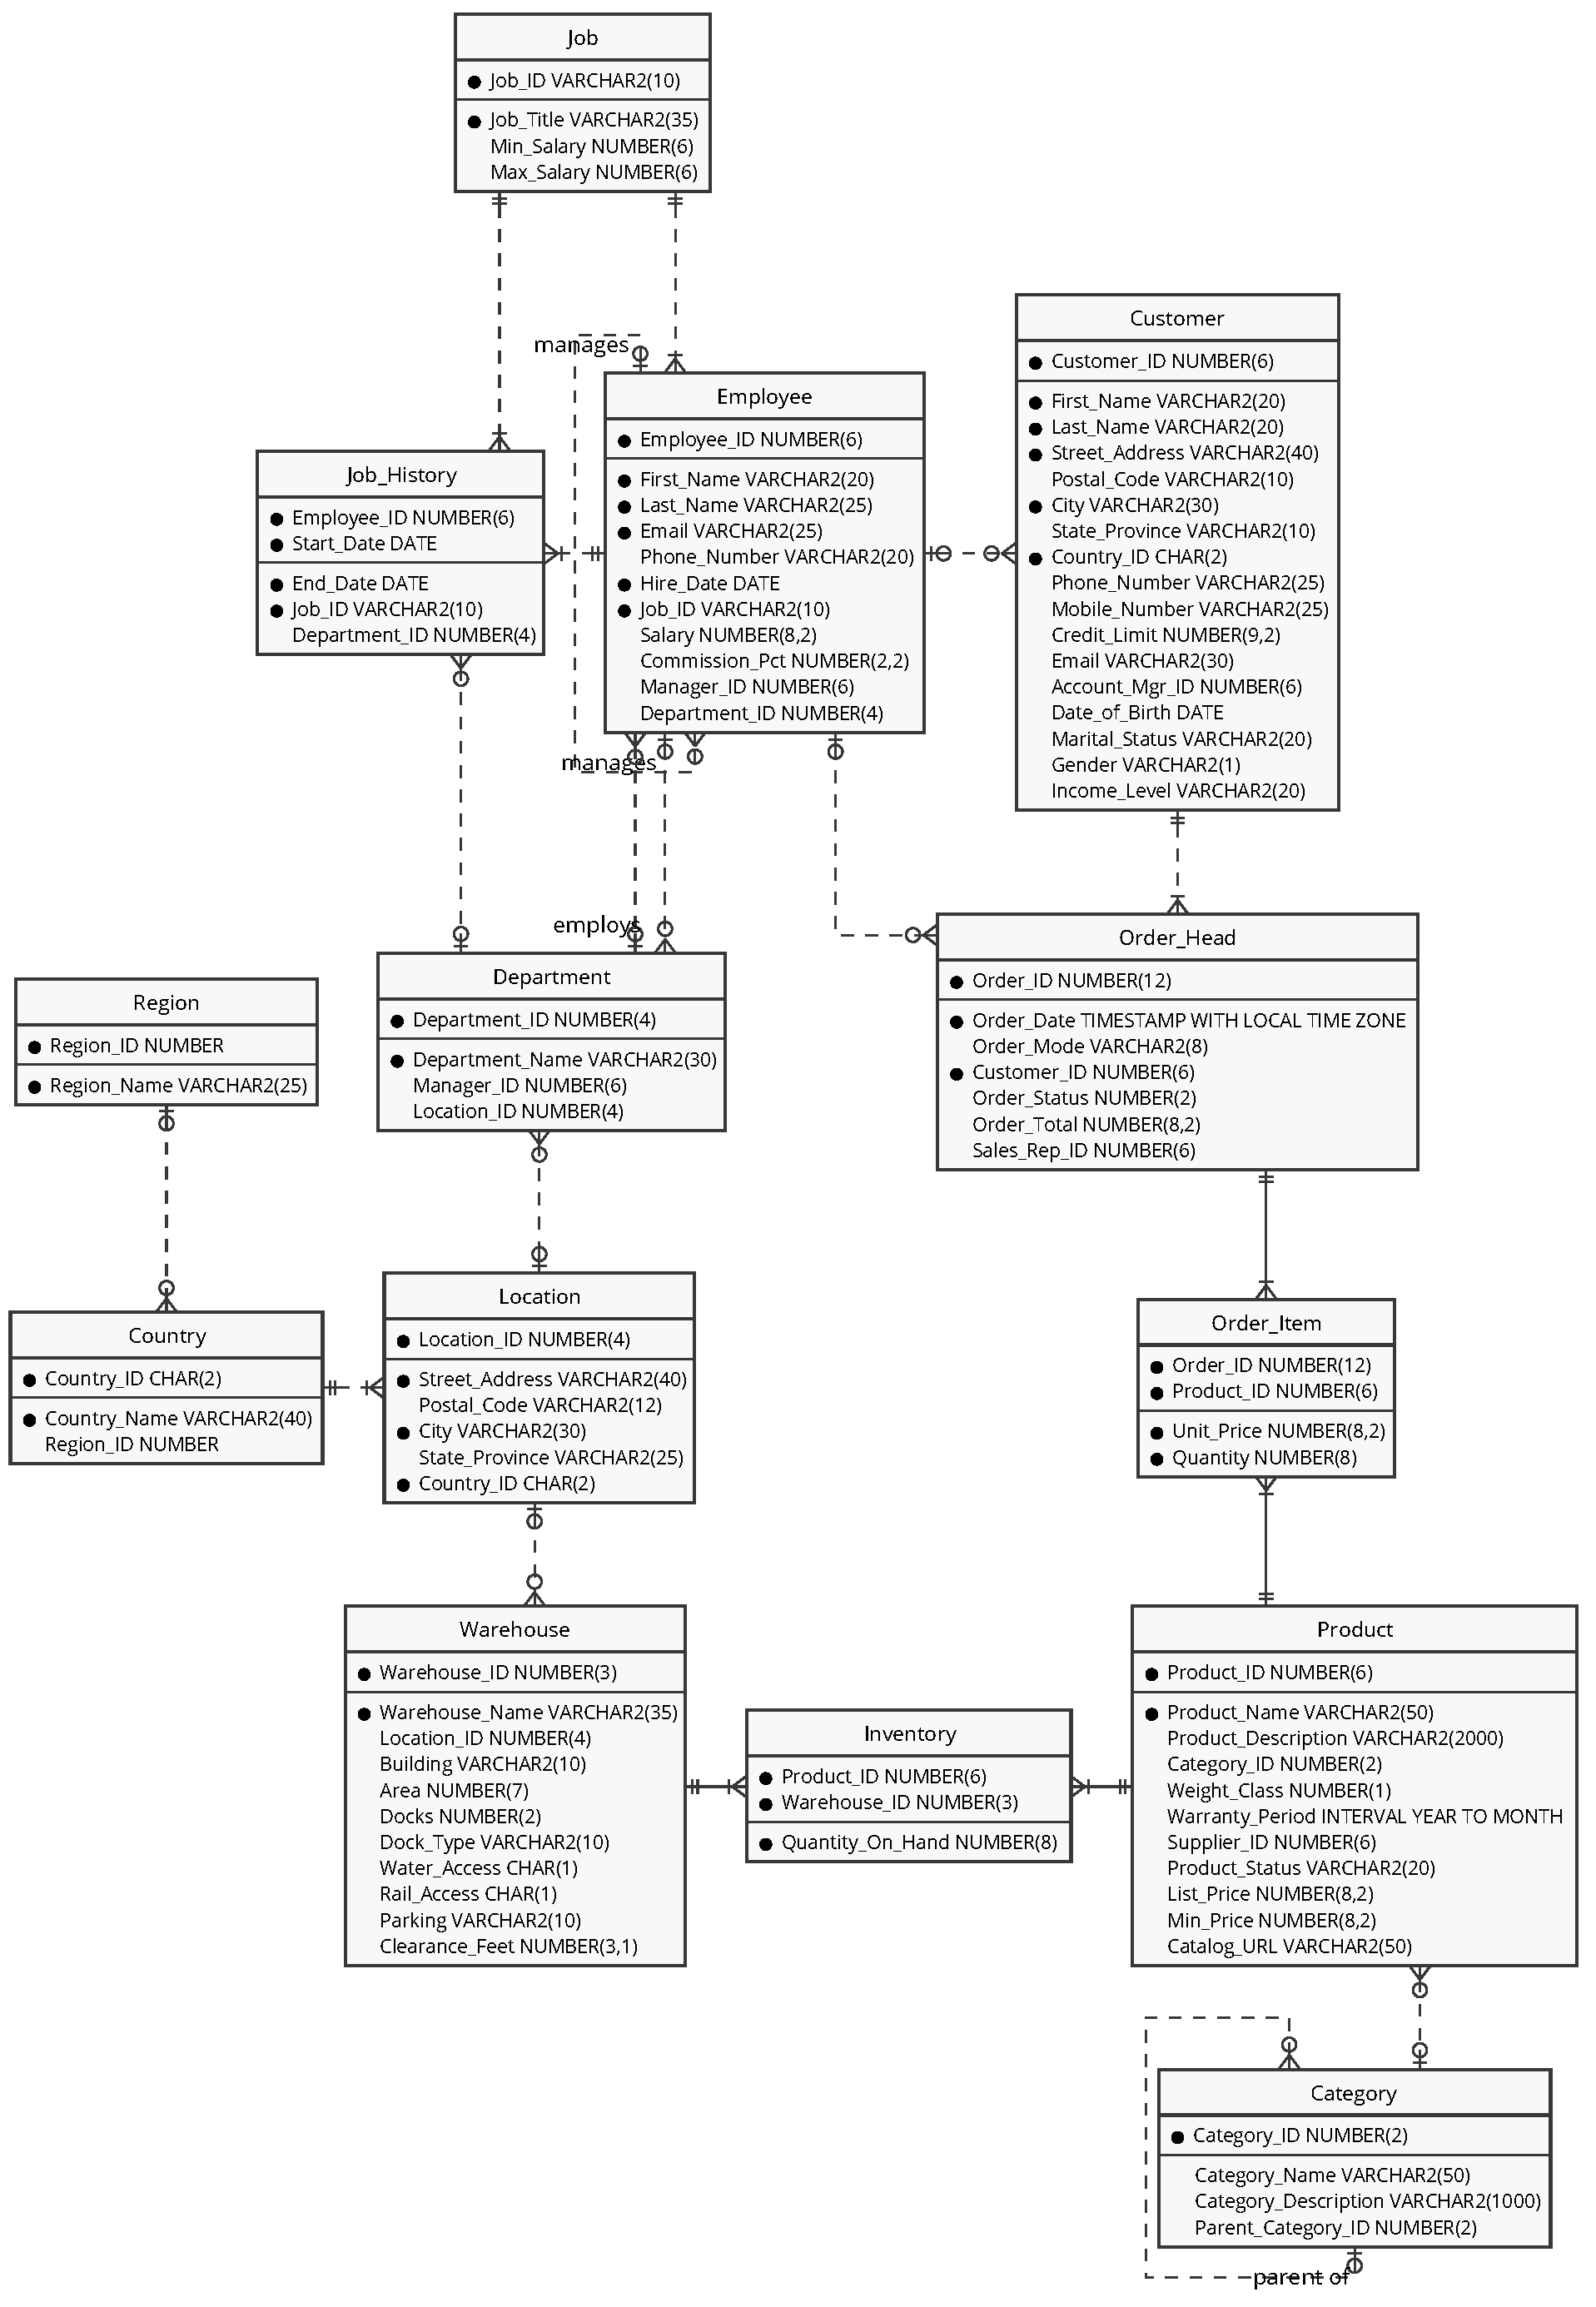
\includegraphics[width=3.25cm,keepaspectratio]{HR_OE_ERD}};
                \node[right=7.5mm of erd] (excel) {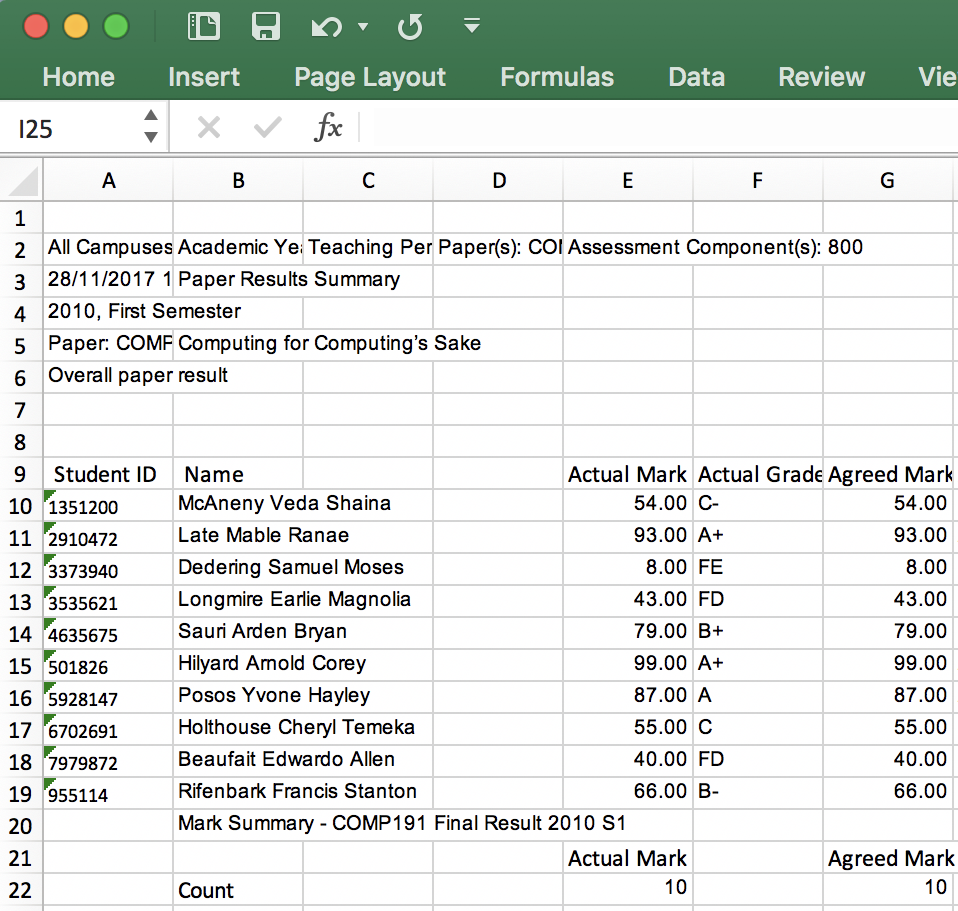
\includegraphics[width=3.25cm,keepaspectratio]{fake_results_excel}};
                \node[right=7.5mm of excel] (web) {
\includegraphics[width=3.25cm,keepaspectratio]{web_page}};
                
                \node[below=0mm of web.south] (weblabel) {free-form};
                \node (excellabel) at (excel |- weblabel) {more flexible};
                \node (erdlabel) at (erd |- weblabel) {formal, “fixed”};
                
                \node[below=-3pt of erdlabel] (erdtext) {\tiny e.g., SQL databases};
                \node[below=-3pt of excellabel] (exceltext) {\tiny e.g., JSON, XML, Excel, …};
                \node[below=-3pt of weblabel] (webtext) {\tiny e.g., email, MS Word, web pages, …};
                
                \path[fill, OU red, ultra thick, nearly transparent] (erd.west) -- ++(0,1cm) -- ($(web.west) + (0,1cm)$) -- ++(0,1cm) -- (web.east) -- ($(web.west) - (0,2cm)$) -- ++(0,1cm) -- ($(erd.west) - (0,1cm)$) -- cycle;
            \end{tikzpicture}
        \end{column}
    \end{columns}
\end{frame}


%%%%%%%%%%%%%%%%%%%%%%%%%%%%%%%%%%%%%%%%%%%%%%%%%%%%%%%%%%%%%%%%%%%%%%%%%%%%%%%%


\begin{frame}
    \frametitle{Moving data around leads to … trouble}
    
    \bigskip
    \centering
    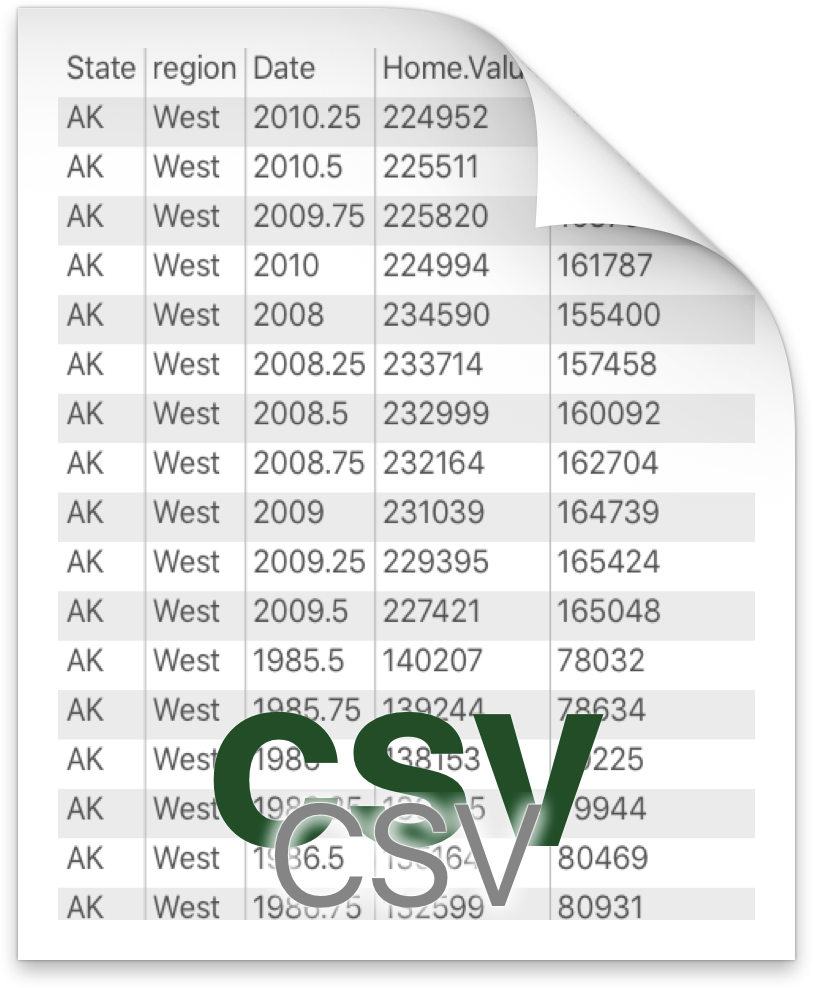
\includegraphics[height=6cm,keepaspectratio]{CSV}
\end{frame}


%%%%%%%%%%%%%%%%%%%%%%%%%%%%%%%%%%%%%%%%%%%%%%%%%%%%%%%%%%%%%%%%%%%%%%%%%%%%%%%%


\begin{frame}
    \frametitle{Project 1: CoreScan (completed)}
    
    \bigskip
    \begin{itemize}
        \item Statistical analysis of body composition data in R.
        
        \item Data exported directly from DXA machine.
        
        \item Relatively straightforward:
        \begin{itemize}
            \item Excel with well-defined columns
            \item some minor cleaning
        \end{itemize}
        
        \item “The way things should be”.
    \end{itemize}
    
    \begin{tikzpicture}[remember picture, overlay]
        \node[above right=5mm of current page.south west)] (ref) {
            \scriptsize\parbox{\columnwidth}{Meredith-Jones, K., Haszard, J., Stanger, N., and Taylor, R. “Precision of DXA-derived visceral fat measurements in a large sample of adults of varying body size.” \emph{Obesity} \textbf{26}(3):505–512. doi:~10.1002/oby.22108}
        };
    \end{tikzpicture}
\end{frame}


%%%%%%%%%%%%%%%%%%%%%%%%%%%%%%%%%%%%%%%%%%%%%%%%%%%%%%%%%%%%%%%%%%%%%%%%%%%%%%%%


\begin{frame}
    \frametitle{Now what?}
    
    \begin{itemize}
    
        \item \todo{}
        
    \end{itemize}
\end{frame}


%%%%%%%%%%%%%%%%%%%%%%%%%%%%%%%%%%%%%%%%%%%%%%%%%%%%%%%%%%%%%%%%%%%%%%%%%%%%%%%%


\begin{frame}
    \centering\Huge
    \structurebf{Questions?}
\end{frame}


%%%%%%%%%%%%%%%%%%%%%%%%%%%%%%%%%%%%%%%%%%%%%%%%%%%%%%%%%%%%%%%%%%%%%%%%%%%%%%%%


\end{document}

Three projects run the gamut from fairly exemplary through to awful.

Project 1: CoreScan (completed)
Meredith-Jones, K., Haszard, J., Stanger, N., and Taylor, R. Precision of DXA-derived visceral fat measurements in a large sample of adults of varying body size. Obesity, 26(3):505–512. doi: 10.1002/oby.22108

• body composition data acquired from dual-energy X-ray absorptiometry (DXA) using GE’s new CoreScan algorithm
• statistical processing in R to compute precision error, etc., using standard methods for the discipline
• relatively straightforward (original data an Excel file with well-defined columns)
• some minor cleaning (duplicate participant entries)
• “the way things should be”


Project 2: student data
• much work around University needs or can use student-related data
    • teaching
    • HE research
    • administration
• teaching & admin
    • student & enrolment data (class lists, email lists, internal assessment, terms)
    • timetable data (streaming, rooms)
    • results data (mainly for proofing and submitting)
• CALT project about data-driven course advising
    • enrolment data for who does what papers and when
    • student data for demographics (ethnicity, gender)
    • paper data for workload (points, EFTS)
    • completion data (of degrees)
    • results data (grades, GPA)
    • one potential output is a tool that illustrates student progression (show medical animation example)
    • needs enrolment data in a graph form (each node represents a paper and each edge represent a transition between papers)
• work currently under review (ICCE) on automated SQL DDL marking system
    • results and internal assessment data across several years for one 200-level paper
• where do these data come from?
    • mostly eVision, via Business Objects (shudder)
        • usually either human readable (PDF) or somewhat machine-readable (CSV, XLS)
        • CSV output often ineffective (empty file)
    • perhaps Blackboard if you’re using that for internals
        • exports as “.xls.csv” (!)
    • EXRPT11 (internal assessment and/or overall results, depending on whether Results I or II)
        • printable version (PDF)
        • data version (Excel)
        • bizarrely, the printable version (when generated as Excel) is easier to process than the data version!
    • SDRPT12 (student retention, including degree completion and yearly workload)
        • only other source is student transcript, which can be generated en masse but aren’t easily machine-readable
        • was completely bustificated until fairly recently (empty columns were collapsed)
    • SDGPA01 for GPA data
    • CARPT004 for some enrolment data
    • TTRPT02 for remaining enrolment data not already in CARPT004 and TTRPT02 (find out what each provides)
    • recent development: LDAP for creating class email lists

• many of Otago’s systems output .xls rather than something more modern
    • ⇒ perservation issues: only reliable tool I’ve found to automatically convert spreadsheet formats to something more permanent is ssconvert (part of Gnumeric)
• no API access
• for a while after eVision came in, the BO reports changed format every few months ⇒ adaptive loading scripts
• reading demlited text files is often easier than other formats (I usually keep the input files in both XLSX and CSV)

• my results management system is consequently a mishmash of bash, Perl, Python, PHP, and R scripts that have been bodged together over time (currently being rewritten frome the ground up in Python)


Project 3: subscription vs. perpetual licensing for consumer-level software
• a lot of work on SaaS vs. perpetual licensing in the corporate world
• consumer software:
    • SaaS (e.g., Google Docs, Office 365)
    • standalone software
        • perpetual license with occasional paid upgrades (still a lot of software)
        • annual subscription (e.g., LetterOpener from 2018 onwards)
        • app store: up-front price (or free) + in-app purchases
    • “software plus a service” (S+aS)
        • either perpetual license or subscription for a service that adds features to the standalone version (e.g., syncing)
        • e.g., 1Password
    • some companies offer more than one of these options
• if we want to compare pricing, we need to get data regarding pricing for historical paid upgrades
    • usually no longer online (they don’t sell that version any more) — with a few exceptions
    • online store fronts have changed over time
    • may be able to extract data from the Wayback Machine (seems to work for the couple I’ve tried), but very manual process


Why are things still like this?
• lack of demand/knowledge/education on the part of data consumers (“you get that with computers”) — don’t realise things could be much better
    • e.g., Heather’s three pages of instructions vs. Mark’s quick and dirty VBA app for generating class email lists
• apathy/lack of response from data providers (e.g., ITS)
    • “we’ll do it if you pay for it”
    • “why would you need that?”
    • “we can’t open up our systems like that — too risky”
    • focused on bigger projects/needs?
• apathy on the part of consumers who do know better
    • usually because they already have workarounds that are “good enough”
• ancient software/interfaces (e.g., Business Objects)
